%%%%%%%%%%%%%%%%%%%%%%% file template.tex %%%%%%%%%%%%%%%%%%%%%%%%%
%
% This is a general template file for the LaTeX package SVJour3
% for Springer journals.          Springer Heidelberg 2010/09/16
%
% Copy it to a new file with a new name and use it as the basis
% for your article. Delete % signs as needed.
%
% This template includes a few options for different layouts and
% content for various journals. Please consult a previous issue of
% your journal as needed.
%
%%%%%%%%%%%%%%%%%%%%%%%%%%%%%%%%%%%%%%%%%%%%%%%%%%%%%%%%%%%%%%%%%%%
%
% First comes an example EPS file -- just ignore it and
% proceed on the \documentclass line
% your LaTeX will extract the file if required
%\begin{filecontents*}{example.eps}
%!PS-Adobe-3.0 EPSF-3.0
%%BoundingBox: 19 19 221 221
%%CreationDate: Mon Sep 29 1997
%%Creator: programmed by hand (JK)
%%EndComments
%gsave
%newpath
%  20 20 moveto
%  20 220 lineto
%  220 220 lineto
%  220 20 lineto
%closepath
%2 setlinewidth
%gsave
%  .4 setgray fill
%grestore
%stroke
%grestore
%\end{filecontents*}
%
\RequirePackage{fix-cm}
%
%\documentclass{svjour3}                     % onecolumn (standard format)
%\documentclass[smallcondensed]{svjour3}     % onecolumn (ditto)
%\documentclass[smallextended]{svjour3}       % onecolumn (second format)
\documentclass[twocolumn]{svjour3}          % twocolumn
%
\smartqed  % flush right qed marks, e.g. at end of proof
%
\newcommand\correspondingauthor{\thanks{Corresponding Author}}
\usepackage{amssymb}% http://ctan.org/pkg/amssymb
\usepackage[utf8]{inputenc} 
\usepackage{graphicx,url} 
\usepackage{array, makecell}
\graphicspath{{img/}}
\usepackage [autostyle, english = american]{csquotes}
\MakeOuterQuote{"}
\usepackage{array, makecell}
\setcellgapes{4pt}
\usepackage[T1]{fontenc}
\usepackage{verbatim}
\usepackage{color}
\usepackage{multirow}
\usepackage{authblk}
\usepackage{cite}

\definecolor{acolor}{rgb}{1,0.5,0}
\newcommand{\dg}{\color{acolor}}
\newcommand{\al}{\color{red}}
\newcommand{\rc}{\color{blue}}

% Para retirar as cores do PDF, basta comentar os três comandos acima e descomentar os abaixo:

%\newcommand{\dg}{}
%\newcommand{\al}{}
%\newcommand{\rc}{}

%
% \usepackage{mathptmx}      % use Times fonts if available on your TeX system
%
% insert here the call for the packages your document requires
%\usepackage{latexsym}
% etc.
%
% please place your own definitions here and don't use \def but
% \newcommand{}{}
%
% Insert the name of "your journal" with
% \journalname{myjournal}
%
\begin{document}

\title{A Brief Survey on Replica Consistency in Cloud Environments
%\thanks{Grants or other notes
%about the article that should go on the front page should be
%placed here. General acknowledgments should be placed at the end of the article.}
}
%\subtitle{Do you have a subtitle?\\ If so, write it here}

%\titlerunning{Short form of title}        % if too long for running head

\author{Robson A. Campêlo \and Marco A. Casanova \and Dorgival Guedes \and Alberto H. F. Laender
}

%\authorrunning{Short form of author list} % if too long for running head

\institute{Robson A. Campêlo \and Dorgival Guedes \and Alberto H. F. Laender \at
              Department of Computer Science, Universidade Federal de Minas Gerais, 31270-901 Belo Horizonte, MG, Brazil \\
              \email{\{robson.campelo, dorgival, laender\}@dcc.ufmg.br}           %  \\
%             \emph{Present address:} of F. Author  %  if needed
           \and
           Marco A.Casanova \at
               Department of Informatics,   Universidade Católica do Rio de Janeiro,  22451-900 Rio de Janeiro, RJ, Brazil \\  \email{casanova@inf.puc-rio.br}   
}

\date{Received: date / Accepted: date}
% The correct dates will be entered by the editor


\maketitle

\begin{abstract}
Cloud computing is a general term that involves delivering hosted services over the Internet. With the accelerated growth of the volume of data used by applications, several organizations have moved their data into cloud servers to provide scalable, reliable and highly available services. A particularly challenging issue that arises in the context of cloud storage systems with geo\-graphi\-cally-distributed data replication is how to reach a consistent state for all replicas. This survey reviews major aspects related to consistency issues in cloud data storage systems, categorizing recently proposed methods into three catego\-ries: (1)~static consistency methods, (2) dynamic consistency methods and (3) consistency monitoring methods.
\keywords{Replica consistency \and Cloud environments \and Storage systems \and Consistency models}
% \PACS{PACS code1 \and PACS code2 \and more}
% \subclass{MSC code1 \and MSC code2 \and more}
\end{abstract}

\section{Introduction}
\label{intro}
%Cloud computing is a general term that involves delivering hosted services over the Internet. The term ``cloud'' is an abstraction of this new model that arose from a network connectivity architecture involving several {\al data} providers stored in external servers.

Cloud computing is a general term that includes the idea of delivering hosted services over the Internet. The term ``cloud'' is an abstraction of this new model that arose from a common representation of a network, since the particular location of a service is not relevant, which means that services and data providers are seen as existing ``in the network cloud''.

In recent years, cloud computing has emerged as a paradigm that attracts the interest of organizations and users due to its potential for cost savings, unlimited scalability and elasticity in data management. In that paradigm, users acquire computing and storage resources in a pricing model which is known as \emph{pay-as-you-go}~\cite{Al-Roomi13}. According to that model, IT resources are offered in an unlimited way and the payment is made according to the actual resources used for a certain period, similarly to the traditional home utilities model.


%Cloud deployment models can be grouped into four types: private, public, hybrid and community~\cite{mell2009nist}. In these environments, the services are provided without the users' concern about how this process occurs. 
Depending on the kind of resource offered to the users, cloud services tend to be grouped in the following three basic models: \emph{Software as a Service} (SaaS)~\cite{dubey2007delivering}, \emph{Platform as a Service} (PaaS)~\cite{beimborn2011platform}, and \emph{Infrastructure as a Service} (IaaS)~\cite{bhardwaj2010cloud}. As an exten\-sion of this classification, when the service refers to a database, the model is known as \emph{Database as a Service} (DBaaS)~\cite{curino2011relational}, which is the focus of this survey. Such a model provides transparent mechanisms to create, store, access and update databases. Moreover, the database service provider takes full responsibility for the database administration, thus guaranteeing backup, reorganization and version updates.
%Moreover, the database service provider ensures the entire responsibility of  database adaministration, i.e., database backup, administration, reorganization or migration from one database version without impacting such an organization.

%With the accelerated growth in the volume of data {\al used} by the applications, several organizations have moved their data into cloud servers to provide scalable, reliable and highly available services. Cloud servers enable service providers to store and customize their data across multiple data centers, separating them physically to meet a growing demand. In this way, services can replicate their state among geographically diverse locations and direct the user to the nearest or most recently accessed one. %location. 
%Thus, replication has become an essential feature of this storage model and is extensively exploited in cloud environments \cite{Chang06bigtable:a, Ibrahim12}. Moreover, replication allows users to obtain various features such as fast access, improved performance and high availability.
%
% DG: o parágrafo acima foi reorganizado na forma a seguir:
%
The use of DBaaS solutions enables service pro\-viders to replicate
and customize their data over multiple servers, which can be physically separated, even placed in different data centers~\cite{Xiong:2011}.
By doing so, they can meet growing demands by directing users to the nearest or most recently accessed server. In that way, replication allows them to achieve features such as fast access, improved performance and higher availability. Thus, replication has become an essential feature of this storage model and is extensively exploited in cloud environments~\cite{Chang06bigtable:a, Ibrahim12}.

A particularly challenging issue that arises in the context of cloud storage systems with geo\-graphi\-cal\-ly-distributed data replication is how to reach a consistent state in all replicas. 
%{\dg In the cloud environment, computer failures and network partitions cannot be completely avoided.} 
Enforcing synchronous replication to ensure strong consistency in such an environment incurs in significant performance overheads, due to the increased network latency between data centers~\cite{goel2007data},
and to the fact that network partitions may lead to service unavailability~\cite{Brewer2000}. 
As a consequence, specific models have been proposed to offer weaker or relaxed consistency guarantees~\cite{Vogels:2009}.

Several cloud storage services choose to ensure availability and performance even in the presence of network partitions rather than to offer a stronger consistency model. NoSQL-based data storage environments provide consistency properties in  eventual mode~\cite{Vogels:2009}, which means that all changes to a replicated piece of data eventually reach all its replicas. However, using this type of consistency increases the probability of reading obsolete data, since the replicas being accessed may not have received the most recent writes. This led to the development of adaptive consistency solutions, which were introduced to allow adjusting the level of consistency at run-time in order to improve performance or reduce costs, while maintaining the percentage of obsolete reads at low levels~\cite{chihoub2012harmony, esteves2012quality, Terry:2013}.

A consistency model in distributed environments seeks to guarantee the consistency of an update operation, as well as the access to an updated object. Obtaining the correct balance between consistency and availability is one of the open challenges in cloud computing~\cite{Elbushra:2014}. In this survey, we focus on state-of-the-art  methods for consistency in cloud environments. Considering the different solutions, we categorize those methods into three distinct categories: (1) static consistency methods, (2) dynamic consistency methods and (3) consistency monitoring methods. Other surveys on distinct issues related to %data
{\al replica} consistency have been recently published~\cite{agrawal2015taxonomy,viotti2016consistency}. We refer the reader to them for further considerations on this topic. 

The remainder of this survey is organized as follows. In Section~2, we present general concepts related to cloud database management. In Section~3, we approach the main consistency models adopted by existing distributed storage systems. 
%In Sections 4 and 5, respectively, we present a taxonomy proposed to categorize the {\al  most prominent} consistency methods {\al found in the literature} and overview {\al each one} of them.
In Section~4, we first propose a taxonomy to categorize the most prominent consistency methods found in the literature and then present an overview of the main approaches adopted to implement them. In Section~5, we provide a sum-up discussion emphasizing the main aspects of the surveyed methods.
%we discuss the methods} we have surveyed. 
Finally, in Section~6, we conclude the survey by summarizing its major issues.

\section{Cloud database %Consistency 
	management}
\label{sec:1}
In this section, we present general concepts related to cloud database management in order to provide a better understanding of the key issues that affect replica consistency in cloud environments. 
Initially, 
% we approach the architectural aspects of the DBaaS model. After that, %Linha retirada com a remoção da sub-seção a seguir
we highlight the cloud storage infrastructure requirements and describe the ACID properties. Then, we introduce the CAP theorem and discuss its associated trade-offs. 

\begin{comment}
\subsection{Data Replication and Data Partitioning Aspects of the DBaas Model}

In the DBaaS model, the architecture is often distributed and data can be stored in possibly hundreds of machines, where the resources are shared among the clients~\cite{Xiong:2011}. As previously mentioned, one of the techniques used to obtain specific features such as fast access, improved performance and high availability is to fully replicate data in geographically distinct locations.  

For example, in a scenario in which a failure occurs in one replica, the system possibly can continue to operate by directing  requests to the other replicas. 

Another benefit is scalability, which allows the system to handle an increase in the number of requests as well as in the volume of stored data~\cite{tanenbaum:2007}. When considering the possibility of data replication in geographically distant areas, it is necessary to define how updates will be spread among the replicas, since the manner how this operation is executed directly affects  replica consistency.

Data partitioning represents another distribution method in the DBaaS model. It is performed by breaking a table into two or more fragments or partitions, which can be stored in different locations~\cite{RahimiHaug:2010}. This method differs from replication in the sense that instead of copying the data it splits them according to certain criteria. 
In cloud environments, partitioning may occur dynamically and in real time.
\end{comment}

\subsection{Cloud data storage requirements}
\label{sec:2.1}
A trustworthy and appropriate data storage infrastructure is a key aspect to %achieve 
provide an adequate cloud data storage infrastructure, 
%data\-base management, 
so that all resources can be efficiently used and shared to reduce consistency issues. Next we list some crucial requirements that must be considered by a shared infrastructure model~\cite{Brewer2000, ju2011survey, rimal2009taxonomy}. \\

\noindent
\textbf{Automation.} The data storage must be automated to be able to quickly execute infrastructure changes required to maintain replica consistency with no human intervention.
%necessary to meet the previous requirements without human intervention.

\noindent
\textbf{Availability.} The data storage must ensure that data continues to be available at a required level of performance in situations ranging from normal to adverse.

\noindent
\textbf{Elasticity.} Not only must the data storage be able to scale with increasing load, but it must also be able to adjust to reductions in load by releasing cloud resources, while guaranteeing compliance with a Service Level Agreement (SLA).
%The data storage must enable a rapid adjustment of {\al its} infrastructure to {\al deal with} the increasing demand and {\dg guarantee} the compliance with any Service Level Agreements (SLAs).

\noindent
\textbf{Fault tolerance.} The data storage must be able to recover in case of failure, \emph{e.g.}, by providing a backup instance of the application that will be ready to take over without disruption.

\noindent
\textbf{Low latency.} The data storage must handle latency issues by measuring and testing the network latency before committing an application. 

\noindent
%\textbf{Partitionability.}
\textbf{Partition  tolerance.} The data storage must be tolerant to  network partitions, \emph{i.e.}, the system must continue to operate despite them. %%~\cite{Brewer2000}.

\noindent
\textbf{Performance.} The data storage must provide an infrastructure that supports fast and robust data access, update and recovery.

\noindent
\textbf{Reliability.} The data storage must ensure that the data can be recovered in case a disaster occurs.

\noindent
\textbf{Scalability.} The data storage needs to quickly scale to meet workload demands, thus providing horizontal and vertical scalability. Horizontal scalability  refers to the ability to increase capacity by adding more machines or setting up a new cluster or a new distributed environment. Vertical scalability, on the other hand, refers to the increase of capacity by adding more resources %such as more memory or an additional CPU,  
to a machine (\emph{e.g.}, more memory or an additional CPU).


\subsection{The ACID properties}

Conventional Database Management Systems must conform to four transaction properties: \textit{Atomicity}, \textit{Consistency}, \textit{Isolation} and \textit{Durability}. Known as the ACID properties, they are well discussed in the literature~\cite{acid1983}, which describes several approaches to achieve them. However, in the DBaaS model, due to the architectural aspects previously described, assuring the ACID {properties} is a nontrivial task. 

Despite the difficulty to ensure the ACID properties in a cloud data storage, strategies have been proposed in an attempt to manage them in web application transactions. For instance, atomicity might be guaranteed by implementing the two-phase commit (2PC) protocol~\cite{gray1978dbos}, whereas isolation can be obtained by a multi-version concurrency control %(MVCC) 
or by a global timestamp, 
and durability %can be achieved 
by applying queuing strategies such as FIFO (\emph{First-In, First-Out}) to concurrent write transactions, so that old updates do not override the latest ones~\cite{Wei:2009}. 
However, replication represents an important obstacle to guarantee consistency.~\cite{Abadi09}. 
Thus, maintaining a replicated database in a mutually consistent state implies that, in all of its replicas, each of their data items must have identical values.~\cite{OzsuValduriez:2011}. 
Therefore, strategies for data update and propagation must be implemented to ensure that, if a copy is updated, all others must also be updated~\cite{tanenbaum:2007}.

\subsection{The CAP theorem}
\label{sec:2.3}
%Brewer \cite{Brewer2000} introduced the CAP theorem, which was subsequently proved by Gilbert and  Lynch~\cite{Gilbert:2002}. 
The CAP theorem was introduced by Brewer as a conjecture~\cite{Brewer2000} and subsequently proved (in  a restricted form) by Gilbert and  Lynch~\cite{Gilbert:2002}. 
Since then it has become an important concept in cloud systems~\cite{brewer2012}.
It establishes that, when considering the desirable properties of \textit{Consistency}, \textit{Availability} and %\textit{Partitionability}
\textit{Partition  tolerance}
%\footnote{Tolerance to any network partition ~\cite{Brewer2000}.  
%\textit{Partition tolerance} occurs when the system continues to operate despite network partitions~\cite{Brewer2000}.}} 
in distributed systems, at most two of them can be achieved simultaneously. 
%{\rc textit{Partition tolerance} occurs when the system continues to operate despite network partitions~\cite{Brewer2000}.} 
%\textbf{NOTA (AL): O conceito de ``partition tolerance'' também é denominado na literatura de ``partitionability''. Assim, devemos incluí-lo na lista anterior, removendo a nota de pé-de-página abaixo. Entretanto isso afeta a Tab.~1, mas não me parece ser um problema difícil de ser resolvido.} 

It is evident that 
%the implications of the CAP theorem introduced conflicts and
the CAP theorem introduces conflicts and imposes several challenges to dis\-trib\-uted systems and service providers. Among the conflicts derived from it, considering that network partitions are inevitable in a geographically distributed scenario, we highlight the trade-off between Consistency and Availability~\cite{gilbert2012perspectives}. 
To illustrate this situation, in Figure~\ref{fig:figure1} we observe that User~2 performs a read request for data item D1 in replica R3 (Da\-ta\-center~2), after User~1 has updated data item D1 in replica R1 (Datacenter~1) in the presence of a network partition that isolates the two data centers. Assuming that the update made by User~1 has not been propagated, there are two possible scenarios: the replicas may be available and User~2 will read obsolete data, thereby violating consistency, or User~2 must wait until the network partition is fixed and the update has been propagated to replica R3, thus violating availability.

%as required. Don't forget to give each section
%and subsection a unique label (see Sect.~\ref{sec:1}).

\begin{figure}[h]
	\vspace{-3mm}
\centering	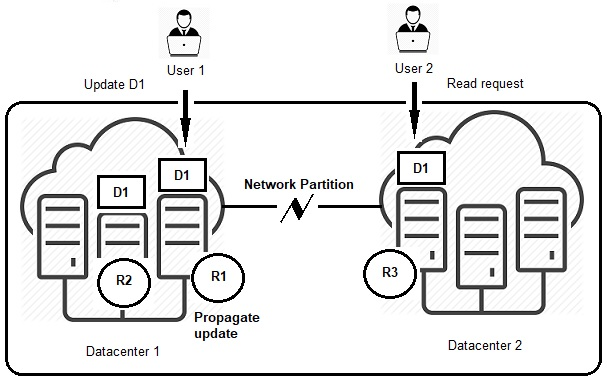
\includegraphics[width=0.48\textwidth]{fig1.png}
	\caption{Consistency vs. Availability in Replicated Systems.}
	\label{fig:figure1}
\end{figure}

The trade-offs caused by the CAP theorem led to the proliferation of not-ACID systems for building cloud-based applications, {\it i.e.,} systems that are {\it basically available}, rely on the maintenance of a {\it soft-state} that can be rebuilt in case of failures and are only {\it eventually consistent} to be able to survive network partitions. Such not-ACID systems, known as BASE~\cite{sosp1997base}, offer distinct consistency models, which are discussed next.

\section{Consistency models}

%In this section, \textbf{we address the consistency models usually adopted by} distributed storage systems.
%we present the concepts of the consistency models in distributed storage systems.
%\textbf{First, we highlight the consistency perspectives} in this environment, and then we provide a hierarchical overview of the main consistency models.

%\subsection{Perspectives on Consistency}
%\subsection{Consistency Perspectives}

A {\it consistency model} may be defined as a contract between a data storage system and the data processes that access it~\cite{tanenbaum:2007}, 
%%It defines strategies for supporting
thus defining strategies that support consistency within a distributed data storage system. However, trade-offs due to the CAP theorem require choosing from a range of models to address different consistency levels, which may vary from a relaxed model to a strict one~\cite{bermbach2013consistency}. 
In this context, there are two distinct perspectives to be considered in a distributed data storage system with respect to consistency~\cite{tanenbaum:2007}: 
the \textit{data-centric perspective} and the \textit{client-centric perspective}.
%the \textit{data provider {\rc perspective}} and the \textit{client {\rc perspective}}.
%In this context, there are two perspectives \textbf{in terms of consistency} to be considered in a distributed storage system \cite{tanenbaum:2007}: the \textit{provider} and the \textit{client}.
%demanding of the systems the need to incorporate a range of models that address consistency guarantees that varying from a relaxed consistency model to a strict consistency model \cite{bermbach2013consistency}. 
%In this context, there are two perspectives to be considered on consistency in a distributed storage system \cite{tanenbaum:2007}: the provider and the client.

From the data-centric perspective, the operations from all processes that want to access the data must be synchronized and ordered to guarantee correct results. From the client-centric perspective, it is often the case that shared updates are rare and mostly access private data. In such cases, the major concern is to make their own operations consistent, which may be simpler to achieve.

%{\al The provider is responsible for synchronizing the processes {\dg that want to access} the replicas and ordering their operations.}
%%the synchronization processes among the replicas and the ordering of the operations. 
%The other perspective refers to the process of interaction between the client and the storage system. 

%These two consistency perspectives are called \textit{data-centric} and \textit{client-centric}~\cite{tanenbaum:2007}. Next, we discuss the consistency models related to each {\rc one of these} perspectives.

\subsection{Data-centric consistency models}

In this perspective, the consistency models seek to ensure that the data access process follows certain rules that guarantee that the storage system works correctly. The period between the update and the moment when this guarantee is reached is called \textit{inconsistency window}. These rules are based on the definition of the results that are expected after read and write operations, even considering that those operations are concurrently performed. However, the absence of a global clock makes the identification of the last write operation a difficult task, which requires some restrictions on the data values that can be returned by a read operation, thus leading to a range of consistency models.  %%~\cite{tanenbaum:2007}.
The consistency models that fall in this category are~\cite{tanenbaum:2007}: \textit{weak consistency, PRAM consistency, causal consistency, sequential consistency} and \textit{strict consistency}. \\
%%We describe these models next. 
%Notice that the last two models  only exist in conventional database management systems and are included here for completeness. 

\noindent \textbf{Weak Consistency.} 
%The weak consistency model offers the lowest possible ordering guarantee. As this guarantee is very weak, we can say that it does not really exist, since an implementation may or may not have a protocol to synchronize replicas.
As its name indicates, weak consistency is the model that offers the lowest possible ordering guarantee, since it allows data to be written across multiple nodes and always returns the version that the system finds first.
%{\rc Basically, it is a model in which a read operation, when data is written across multiple nodes, returns the version that the system finds first, no matter it is the most recent one or not.}
This means that there is no guarantee that the system will eventually become consistent,
%Thus, this model provides consistency to a group of transactions instead of to individual reads and writes, 
which is the case of the stricter consistency models discussed next (PRAM, causal, sequential and strict)~\cite{tanenbaum:2007,Vogels:2009}. \\

\noindent \textbf{PRAM Consistency.}
PRAM (Pipelined Random Access Memory) consistency, also known as FIFO consistency, is a model in which write operations from a single process are seen by the other processes in the same order that they were issued, whereas writes from different processes may be seen in a different order by different processes. In other words, there is no guarantee on the order in which the writes are seen by different processes, although writes from a single source must keep their order as if they were in a pipeline~\cite{lipton1988pram,tanenbaum:2007}. \\

\noindent \textbf{Causal Consistency.}
Causal consistency is a mod\-el in which a sequential ordering is always maintained only between requests that have a \textit{causal dependency}. Two requests have a causal dependency if at least one of the following two conditions is achieved: (1) both requests are executed on a single thread and the execution of one precedes the other in time; (2) request B reads a value that has been written by a request A. Moreover, this dependency is transitive, so if A and B have a causal dependency, and B and C also have a causal dependency, then there is also a causal dependency between A and C~\cite{tanenbaum:2007,Vogels:2009}.
%However, concurrent requests do not share this property. In this case, all requests must be serialized in the same order on all replicas~\cite{tanenbaum:2007}. 
%%% A condição acima é usada para transformar ord. causal em ord. total.
Thus, in a scenario of an always-available storage system in which requests have causal dependencies, a consistency level stricter than that provided by the causal model cannot be achieved due to trade-offs of the CAP theorem~\cite{abadi2012consistency,mahajan2011consistency}. \\
%Causal consistency is a model in which a sequential ordering is always maintained only between requests that have a causal relationship. Thus, concurrent requests do not share this relationship. In this case, all requests must be serialized in the same order on all replicas \cite{tanenbaum:2007}. Thus, in a scenario of an always-available storage system in which requests have causal dependencies, a consistency level stricter than that provided by the causal model cannot be achieved due to trade-offs of the CAP theorem~\cite{mahajan2011consistency}.

%More specifically, two requests have a causal dependency if at least one of the following two conditions is achieved: (1) both requests are executed on a single thread and the execution of one precedes the other in time; (2) if a request B reads a value that has been written by a request A. Moreover, the relationship is transitive, so if A and B have a causal relation, and B and C also have a causal relation, then A and C share the same relationship~\cite{tanenbaum:2007, Vogels:2009}.
%\vspace{1mm}

\noindent \textbf{Sequential Consistency.}
Sequential consistency is a stricter model that differs from the previous one in the sense that it extends to all requests the need of the replicas to agree on the ordering of non-causally related requests. It requires  that all operations be serialized in the same order in all replicas and also that those related to the same process are executed in the order that they are received by the storage system~\cite{tanenbaum:2007}. \\
%{\rc This model requires that the same serialization order imposed by the requests (verificar esta desri\c{c}\~ao)} is maintained on all replicas and the storage system must execute the requests in the order that they are received if they were sent by the same client~\cite{tanenbaum:2007}.
%\vspace{2mm}

\noindent \textbf{Strict Consistency.}
Strict consistency is a mod\-el that provides the strongest consistency level. It states that if a write operation is performed on a data item, the result needs to be instantaneously visible to all processes, regardless of in which replica the operation occurred. To achieve that, an absolute global time order must be maintained~\cite{tanenbaum:2007}.

\subsection{Client-centric consistency models}

In this perspective, a distributed data store is characterized by a relative absence of simultaneous updates.
%Also, when a simultaneous update occurs, the solution of any concurrency problem is simple to achieve.
%{\al Thus, in case that updates occur, there is no need to resolve them.}
%there are no problems in resolve them. 
The emphasis is then to maintain a consistent view of data items for an individual client process that is currently operating on the data store. 
The consistency models that fall in this category are~\cite{tanenbaum:2007}: \textit{eventual consistency, monotonic reads consistency, monotonic writes consistency, read-your-writes consistency} and \textit{writes-follow-reads consistency}. \\
%{\rc We describe each one of these consistency models next.}

\noindent \textbf{Eventual Consistency.}
The eventual consistency mod\-el states that all updates will propagate through the system and all replicas will gradually become consistent, after all updates have stopped for some time~\cite{tanenbaum:2007, Vogels:2009}. Although this model does not provide concrete consistency guarantees, it is advocated  as a solution for many practical situations~\cite{BailisVFHS12,BailisVFHS14,balegas2015putting,Chihoub2014,Vogels:2009} and has been implemented by several distributed storage systems~\cite{Chang06bigtable:a, decandia2007dynamo, Ghemawat2003Google, lakshman2010cassandra}. \\

\noindent \textbf{Monotonic Read Consistency.}
The monotonic read consistency model guarantees that if a process reads a version of a data item \textit{d} at time \textit{t}, it will never see an older version of \textit{d} at a later time. In a scenario where data visibility is not guaranteed to be instantaneous, at least the versions of a data item will become visible in chronological order~\cite{tanenbaum:2007,Vogels:2009}. \\

\noindent \textbf{Monotonic Write Consistency.}
This model guarantees that a data store must serialize two writes \textit{$w_{1}$} and \textit{$w_{2}$} in the same order that they were sent by the same client~\cite{tanenbaum:2007, Vogels:2009}. 
For instance, if the initial write operation \textit{$w_{1}$} is delayed, it is not allowed for a subsequent write \textit{$w_{2}$} to overwrite that data item before \textit{$w_{1}$} completes. \\

\noindent \textbf{Read-Your-Writes Consistency.}
%The read-your-writes 
This consistency model is closely related to the monotonic read one. It guarantees that once a write operation is performed on a data item \textit{d}, its effect will be seen by any successive read operation performed on \textit{d} by the same process~\cite{tanenbaum:2007, Vogels:2009}. This means that if a client has written a version \textit{v} of a data item \textit{d}, it will always be able to read a version at least as new as \textit{v}. \\
%or upper.

\noindent \textbf{Writes-Follow-Reads Consistency.} %The writes-follow-reads 
This consistency model guarantees that if a write operation \textit{w} is requested by a process on a data item \textit{d}, but there has been a previous read operation \textit{r} on \textit{d} by the same process, then it is guaranteed that \textit{w} will only be executed on the same or more recent value of \textit{d} previously  read.~\cite{tanenbaum:2007}. 

\begin{comment} %%%%%%%%%%%%%%%%%%%%%%%%%%%%%%%%
\subsection{Hierarchical View of the Consistency Models}
%https://www.overleaf.com/8967554ryqqdyzyrdcp#
In order to achieve a better understanding of the relationships among the consistency models, they can be hierarchically organized according to their degree of strictness from a lower consistency level to a higher one (see Figure~\ref{fig:hierarchicalView}).  

\begin{figure}[h]
\centering	\includegraphics[width=0.48\textwidth]{fig2b.jpg}

%\vspace{-3mm}
\caption{Hierarchical View of the Consistency Models.}
\label{fig:hierarchicalView}
\end{figure}
\vspace{-1mm}

This hierarchical organization also considers some model combinations, such as the PRAM consistency model that may be seen as a combination of the monotonic read (MR), monotonic write (MW) and read-your-writes (RYW) models~\cite{bailis2013highly}. In addition, according to Brzezi\'nski et al.~\cite{brzezinski2004session}, there is also a relationship between causal consistency, which is a data-centric model, and the client-centric perspective,  
%and apparently, 
thus meaning that causal consistency is similar to write-follows-reads (WFR). 
%\vspace{2mm}
\\
\end{comment}

\section{Replica consistency methods}

%In this section, we survey state-of-the-art methods for consistency in cloud environments.  The survey includes methods that we considered to be among the most representative in the literature.
In this section, we present an overview of state-of-the-art methods for replica consistency in cloud environments. This overview includes those methods that we considered to be among the most representative in the literature.
Based on the similarities of their core ideas, we classified these %%selected 
methods into three distinct categories:~(1) static consistency methods, (2) dynamic consistency methods and (3) consistency monitoring methods. In the following sections, we first describe the generic characteristics of each category and then present an overview of its specific methods.

\begin{comment} %%%%%%%%%%%%%%%%%%%%%%%%%%
In this section, we propose a taxonomy for categorizing the various consistency methods addressed in this survey. {\rc We also present an overview of 
%the main approaches adopted by 
each of them. These methods are among the most representative in the literature, although our survey is not exhaustive.} The proposed taxonomy categorizes these methods as follows: \emph{static consistency methods, dynamic consistency methods, and consistency monitoring methods}. 

Our criteria for proposing this taxonomy are based on the similarities of the core ideas behind the methods, %in which we observed the common aspects in their approaches, 
which led us to consider these three categories as the most representative to categorize them. In what follows, we describe the main characteristics of the methods that belong to each category. 
\end{comment}

\subsection{Static consistency methods}

This category includes those methods that provide consistency guarantees in cloud storage systems, but which are not flexible enough to support self-adaptivity according to the applications' consisten\-cy requirements, \textit{i.e.}, such methods do not offer a diversity of consistency options. Representative methods in this category are of two types: \textit{Event Sequencing-based Consistency} and \textit{Clock-bas\-ed Strict Consistency}. They are described next.

% which have been  imple\-mented  in systems like PNUTS~\cite{cooper2008pnuts}, and  Spanner~\cite{Corbett:2013} and Clock-SI~\cite{Du2013}, respectively.

\subsubsection{Event sequencing-based consistency}

This type of consistency method aims at hiding the replication complexity by providing a consistency model that lies between the two extremes of general serializability and eventual consistency. The key aspect behind this type of method is the observation that 
%serializability os transactions is inefficient
transaction serializability is costly and often unnecessary in web applications~\cite{BailisVFHS14}.

The most representative system that implements this type of method is PNUTS~\cite{cooper2008pnuts}, which is a massively parallel and geographically distributed DBMS developed by Yahoo for web applications. PNUTS developers observed that web applications typically manipulate one record at a time, whereas different records may be located in different geographic  localities. Hence, an event sequencing-based consistency method establishes that all replicas of a given record receive all updates applied to that record in the same order. This strategy is implemented by designating one of the replicas as the master for each record, so that this master receives all writes sent to that record by the other replicas. If a record has the majority of its writes sent to a particular replica, this replica becomes the master for that record.

\subsubsection{Clock-based strict consistency}

Systems that implement this type of consistency method are characterized by the use of clock-based mechanisms to control timestamps to enforce strict consistency~\cite{Corbett:2013, Du2013}. They offer the guarantee that arbitrary objects in the data store are accessed atomically and isolated from concurrent accesses.
%For that, it is provided strong semantics with general purpose transactions, supporting read and write operations.
The approach behind this consistency method is based on the ability of a system to provide a timestamp log to track the order in which operations occur. According to Bravo et al.~\cite{bravo2015use}, this type of technique is implemented by the data storage systems themselves and might impact the consistency guarantees that they provide.
%In some distributed DBMS, a timestamp-based algorithm is used for controlling concurrency allowing to safely handle transactions.

Spanner~\cite{Corbett:2013} and Clock-SI~\cite{Du2013} are representative systems that implement this type of consistency method. The former is a relational-like distributed data store system developed by Google. It assigns globally\--mean\-ingful commit timestamps that reflect the serialization order of the transactions, which may be distributed. Spanner also enforces that if a transaction \textit{T$_{2}$} begins after the commit of a transaction \textit{T$_{1}$}, then the commit timestamp of \textit{T$_{2} $} must be greater than the commit timestamp of \textit{T$_{1}$}.

On the other hand, Clock-SI implements the so called \textit{snapshot isolation}, which is a consistency criterion for partitioned data storage. In this strategy, read-only operations read from a consistent snapshot and other operations perform a commit if no objects written by these transactions were concurrently written. The local physical clock is used by each transaction to identify its read timestamp. Another example of a system that implements \textit{snapshot isolation} is Vela~\cite{salomie2015scaling}. It uses this technique to provide fault tolerance, performance and scalability, without sacrificing consistency.

\begin{comment}  %%%%%%%%%%%%%%%%%%%%%%%%%%%
%This category includes those methods that rely on mechanisms proposed to provide consistency in cloud storage systems that {\al support service-oriented replication or partitioned data storage}. 
This category includes those consistency methods that rely on mechanisms that support service-oriented replication or partitioned data storage.
The predominant characteristic of these methods is that 
%the consistency guarantees 
they are not flexibile enough to support the clients' consistency requirements and, therefore, do not provide a diversity of consistency options. %in accordance to the Service Level Agreement (SLA).  
Representative methods in this category 
%{\rc are \textit{Event Sequencing-based Consistency} (PNUTS~\cite{cooper2008pnuts}) and \textit{Clock-bas\-ed Strict Consistency} (Spanner~\cite{Corbett:2013}, Clock-SI~\cite{Du2013})}.
{\al are of two types: \textit{Event Sequencing-based Consistency} and \textit{Clock-bas\-ed Strict Consistency}, which have been  imple\-mented  in systems like PNUTS~\cite{cooper2008pnuts}, and  Spanner~\cite{Corbett:2013} and Clock-SI~\cite{Du2013},  respectively}.
\end{comment}

\subsection{Dynamic consistency methods}

The methods included in this category implement mechanisms that provide dynamic characteristics such as self-adaptive 
%consistency methods that automatically adjust the degrees of consistency 
or flexible consistency guarantees, which allow the selection or specification of the desired consistency level at any given point. 
These methods are of two types, \textit{Automated and Self-adaptive Consistency} and \textit{Flexible Consistency}, and are described next.

%The first type has been implemented in systems like Harmony~\cite{chihoub2012harmony}, VFC$^3$~\cite{esteves2012quality} and Pileus \cite{Terry:2013}, whereas the second one supports systems like 
%Indigo~\cite{balegas2015putting}, SSOR~\cite{Chen:2014} and Amazon DynamoDB~\cite{sivasubramanian2012amazon}. 

\subsubsection{Automated and self-adaptive consistency}

This type of consistency method aims at dynamically enforcing multiple consistency degrees over distinct data objects. Three main approaches have been adopted to implement such methods. 

%{\rc  probabilistic computation~\cite{chihoub2012harmony}, consistency vector \cite{esteves2012quality} and dynamic server selection}~\cite{Terry:2013}. 

The first approach is based on probabilistic computations that provide an estimation of the stale reads\footnote{ Read operations that return  old instances of a data object that has already been updated to a newer value~\cite{lu2015existential}.} rate. Once the estimation model is computed, it is possible to identify the key parameter that affects the stale reads and then to scale up/down the number of replicas involved in read operations in order to maintain a low tolerable fraction of stale reads. This approach is mainly implemented by Harmony~\cite{chihoub2012harmony}, which is a consistency-based system that aims at gradual and dynamically tuning the consistency level at runtime according to the applications' consistency requirements.

The second approach allows the evaluation and enforcement of divergence bounds over data objects (table/row/column), %so that the 
thus providing consistency levels that can be automatically adjusted based on statistical in\-for\-ma\-tion~\cite{PhansalkarDaniL15}. The evaluation takes place on a divergence vector every time an update request is received, although it is necessary to identify the affected data objects. If any limit is exceeded, all updates since the last replication are placed in a FIFO-like queue to be propagated and executed on the other replicas. 
The most representative system that implements this approach is VFC$^3$ (\textit{Versatile Framework for Consistency in Cloud Computing})~\cite{esteves2012quality}, which provides three-dimensional consistency Qual\-ity-of-Service vectors, where users can specify consistency parameters according to the QoS level desired, thus letting the system automatically adjust the consistency degree.

Finally, the third approach is characterized by dynamically selecting to which server (or even a set of servers) each read of a record must be directed, so that the best service is delivered given the current configuration and system conditions. Hence, this approach is adaptable to distinct configurations of replicas and users, as well as to changing conditions such as variations on the network performance or server load. Another important aspect of this approach is the fact that it allows application developers to provide a Service Level Agreement (SLA) that specifies the applications' consistency/latency desires in a declarative~ manner.  Pileus~\cite{Terry:2013} is a key-value storage system that implements this approach. It provides a diversity of consistency guarantee options for globally distributed and replicated data environments. It also allows several systems or even clients of a system to achieve different consistency degrees, even while sharing the same data.

\subsubsection{Flexible consistency}

This type of consistency method is characterized by its flexibility to adapt to predefined consistency models. In this context, there are four main approaches that implement this type of consistency: (1) combining both weak and strict consistency depending on the operation~\cite{balegas2015putting}, (2) providing configuration options for actors in a multi-cluster~\cite{BernsteinBBCFKK17}, (3) adopting the notion of consistency regions~\cite{Chen:2014} and (4) performing eventually or strongly consistent reads as neededs~\cite{sivasubramanian2012amazon}.

The first approach aims at strengthening eventual consistency, thus allowing the applications to specify consistency rules, or \textit{invariants}, that must be maintained by the system. Once those invariants are defined, it is possible to identify the operations that are potentially unsafe under concurrent execution, thus allowing one to select either a violation-avoid\-ance or an invariant-repair technique. Indigo~\cite{balegas2015putting} is a middleware system that implements this approach. It supports an alternative consistency method built on top of a geo-replicated key-value data store. 

The second approach aims at supporting updates with a choice of linearizable and eventual consistency. GEO~\cite{BernsteinBBCFKK17} is an open-source geo-distributed actor\footnote{Service applications may use actors to provide a programming model to simplify synchronization, fault-tolerance and scalability. It represents a useful abstraction for the middle tier of scalable service applications that run on a virtualized cloud infrastructure in a datacenter~\cite{BernsteinBBCFKK17}.} system that implements this approach. In GEO, an actor may be declared as \textit{volatile} or \textit{persistent}. In the first case, the latest version resides in memory and may be lost when servers fail, where in the second case the latest version resides in the storage layer. In case a user requests linearizability, GEO guarantees true linearizability by applying to the persistent storage in real time in between call and return.

The third approach is based on a formalism proposed to support the applications’ consistency requirements. The trade-off between consistency and scalability requirements is handled by introducing the notion of consistency regions and service-delivery-oriented consistency policies. A consistency region is defined as a logical unit that represents the application state-level requirements for consistency and scalability. This concept is used to define consistency boundaries that separate each group of services that need to be ordered. Hence, services that need to be kept consistent must be associated to a certain region. The definition of what region a service belongs to and which services that can be concurrently delivered is set by the system administrators. 
Scalable Service Oriented Replication (SSOR)~\cite{Chen:2014} is a middleware that implements this approach. It covers three distinct types of consistency region: (1)~Conflict Region (CR), which is a region composed by services that have conflicting requirements for consistency regardless of the session; (2) Sessional Conflict Region (SCR), which is a region that includes services of a particular session with conflicting consistency requirements; and (3) Non-Con\-flict Region (NCR), which is a region that does not impose any consistency constraints or requirements.

Finally, the fourth approach aims at providing elasticity and flexibility in order to handle unpredictable workloads, but allowing a system to be tuned for capacity. Due to this characteristic, it allows applications to perform eventually or strongly consistent reads as needed. Amazon DynamoDB~\cite{sivasubramanian2012amazon} is a highly reliable and cost-effective NoSQL database service that implements this  approach. It was built based on the experience with its predecessor Dynamo~\cite{decandia2007dynamo}. DynamoDB adopts eventual consistency as its default model, which does not guarantee that an eventually consistent read will always reflect the result of a recently completed write. On the other hand, when adopting a stronger consistency model, it returns a result that reflects all writes that have received a successful response prior to that read.

\subsection{Consistency monitoring methods}

Alternatively, instead of directly handling data consistency issues, some methods focus on providing mechanisms that allow data owners to detect the occurrence of consistency violations in the cloud storage. This means that 
%by {\al  using these} methods a group of clients might perform auditing on their data and make decisions based on how the Cloud Service Provider (CSP) stores and manages {\rc all data copies {\al  according to the consistency level that has been agreed upon} in  the service level contract. 
clients might audit their own data and make decisions based on how the Cloud Service Provider (CSP) stores and manages their data copies according to the consistency level that has been agreed upon in  the service level contract. The methods in this category are of two types, \textit{Consistency Verification} and \textit{Consistency Auditing}, and are described next.

%and have been respectively implemented in VICOS~\cite{BrandenburgerCK15}, and in DMR-PDP~\cite{MukundanML12} and CaaS~\cite{liu2014consistency}.

\subsubsection{Consistency verification}

These methods rely on two approaches to consistency verification. The first consists of a protocol that enables a group of mutually trusting clients to detect consistency violations on a cloud storage, whereas the second provides a verification scheme that allows data owners to ensure whether the CSP
%Cloud Service Provider (CSP) 
complies with the SLA for storing data in multiple replicas.

%The protocol is implemented by VICOS
This protocol-based approach is adopted by VICOS (Verification of Integrity and Consistency for Cloud Object Storage)~\cite{BrandenburgerCK15}. VICOS supports the optimal con\-sist\-ency concept of \textit{fork-linearizability}, which captures the strongest achievable notion of consistency in multi-client models. The method may guarantee this notion by registering the causal evolution of the user’s views into their interaction with the server. In case the server creates only a single discrepancy between the views of two clients, it is ensured that these clients will never observe operations of each other afterwards. That is, if these users communicate later and the server ever lies to them, the violation will be immediately discovered. Thus, users can verify a large number of past transactions by performing a single check.

The verification approach is implemented by DMR-PDP~(\textit{Dynamic Multi-Replica Provable Data Possession})~\cite{MukundanML12}. The context addressed by this scheme is that whenever data owners ask the CSP to replicate data at different servers, they are charged for this. Hence, data owners need to be strongly persuaded that the CSP stores all data copies that are agreed upon in the service level contract, as well as that all remotely stored copies correctly execute the updates requested by the users. 
This approach deals with such problems by preventing the CSP from cheating the data storage; for instance, by maintaining fewer copies than paid for. Such scheme is based on a technique called \textit{Provable Data Possession}~\cite{ateniese2007provable}, which is used to audit and validate the integrity and consistency of data stored on remote servers.

\subsubsection{Consistency auditing}

This kind of method is based on an architecture that consists of a large data cloud maintained by a CSP
and multiple small audit clouds composed of a group of users that cooperate on a specific job ({\it e.g.}, revising a document or writing a program). The required level of consistency that should be provided by the data cloud is stipulated by an SLA 
%Service Level Agreement (SLA) 
involving the audit cloud and the data cloud. Once the SLA exists, the audit cloud can verify whether the data cloud violates it, thus quantifying, in monetary terms or otherwise, the severity of the violation.

Consistency as a Service (CaaS)~\cite{liu2014consistency,MathBiradar:2013} implements this method. It relies on a two-level auditing structure, name\-ly: \textit{local auditing} and \textit{global auditing}. Local auditing allows each user to independently perform local tracing operations, focusing on monotonic read and read-your-write consistencies. Global auditing, on the other hand, requires that an auditor is periodically elected from the audit cloud to perform global tracing operations, focusing on causal consistency. This type of method is supported by constructing a directed graph of operations, called the \textit{precedence graph}. If the constructed graph is a directed acyclic graph (DAG), the required level of consistency is preserved~\cite{liu2014consistency}.

\section{Discussion}

\begin{comment}  %%%%%%%%%%%%%%%%%%%%%%%%%%%
{\color{yellow}
\noindent
\textbf{(versão anterior)}\par
In the category of consistency guarantee methods, we have described the \textit{per-record timeline consistency} method \cite{cooper2008pnuts}. This method was designed in order to achieve the Yahoo!’s applications consistency requirements, thus it is based on the experience with many web applications. The main contribution of this method is the conception that in a scenario of replicated data storage in web applications, consistency can be achievable by the control of events (inserts, updates and deletes) in a timeline. This control is based on a sequence number that consists of the generation and the versioning of the record, where each update of an existing record implies a new version. A consistent version from the timeline is returned if a read operation is performed of any replica, which always move forward in the timeline.

The approach of object versioning is also exploited by the clock-based strict consistency method. Clock-SI \cite{Du2013} and Spanner \cite{Corbett:2013} capture similar idea in the ordering of events by the exploitation of clock-based mechanisms in order to keep track of the ordering of transactions.

We observe that the ordering of events is a well-understood approach in distributed systems \cite{fidge1991logical, lamport1978time, mattern1989virtual}. The concept of one event happening before another represents a causal relationship and the total ordering of this events can be used for solving synchronization issues, so that the methods above described extend this concept on their particular approaches.

In the category of consistency auditing methods we have described \textit{consistency verifying protocols}  \cite{BrandenburgerCK15, MukundanML12}   and \textit{consistency auditing}\cite{liu2014consistency}. In general, these methods are suitable for scenarios where multiple clients cooperate on a remotely data stored in a potentially misbehaving service, and they need rely on the cloud service provider regarding the confidentiality and correctness of their data. Furthermore, these clients need to verify if the data updates that are requested are correctly executed on all remotely stored copies, whereas the consistency level required is maintained.

Regarding the dynamic consistency methods there are \textit{automated and self-adaptive consistency} \cite{chihoub2012harmony, esteves2012quality, Terry:2013} and \textit{flexible consistency guarantees} methods \cite{Chen:2014, sivasubramanian2012amazon}. Instead of to apply the same consistency guarantee methods' approach, the automated and self-adaptive are focused in achieve automaticity in their consistency guarantees by the use of mechanisms that adjust the degrees of consistency without human intervention. This is an important feature for applications that have temporal characteristics, which require dynamic adjustment in the consistency requisites of data over time and real-time workload cloud storage systems. Moreover, the flexible guarantees approach seeks to address the applications’ consistency requirements and flexibly adapt to predefined consistency models.
}
\end{comment}

\begin{table*}[t]
	\setlength\extrarowheight{4pt}
	\centering
	\footnotesize{
		\caption{Summary of the Surveyed Replica  Consistency Methods}
		\vspace{1mm}
		\label{tab:surveyedMethods}
		\begin{tabular}{>{\raggedright\arraybackslash}p{2.0cm}>{\raggedright\arraybackslash}p{3.2cm}>{\raggedright\arraybackslash}p{10.5cm}}
			\hline
			Category   & Method    & Brief Description \\ \hline
			Static Consistency & Event Sequencing-based Consistency \cite{cooper2008pnuts} & Establishes that all replicas of a given record apply all updates to a record in the same order. \\                                                   
			& Clock-based Strict Consistency \cite{Corbett:2013, Du2013, salomie2015scaling} & Uses clock-based mechanisms to control timestamps to enforce strict consistency. \\ \hline
			
			Dynamic Consistency  & Automated and Self-Adapt\-ive Con\-sist\-en\-cy \cite{chihoub2012harmony, esteves2012quality, Terry:2013} & Provides a gradually and dynamically tunable consistency level at runtime according to the applications' consistency requirements. \par Enforces increasing degrees of consistency for different types of data, based on their semantics.\\
			& Flexible Consistency Guarantees \cite{balegas2015putting, BernsteinBBCFKK17, Chen:2014, sivasubramanian2012amazon} & Allows applications to specify consistency rules, or \textit{invariants}, that must be maintained by the system. \par Supports updates with a choice between linearizable and eventual consistency. \par Supports the applications' consistency requirements and flexibly adapt to predefined consistency models. \par Allows applications to perform eventually or strongly consistent reads as needed.  \\ \hline
			
			Consistency Monitoring  & Consistency \ \ Verification \cite{BrandenburgerCK15, MukundanML12} & Enables a group of mutually trusting clients to detect data-integrity and consistency violations.  \par Allows the data owner to ensure that the Cloud Service Provider stores all data copies that are agreed upon in the service level contract.  \\
			& Consistency \ \ \ \ \ \ \ \ Auditing \cite{liu2014consistency,MathBiradar:2013} & Implements a Local and Global Auditing structure to allow a group of clients to detect the occurrence of consistency violations.    \\
			\hline
	\end{tabular}}
\end{table*}

As proposed in Section~4, replica consistency methods can be grouped in three categories: static consistency methods, dynamic consistency methods and consistency monitoring methods.

Static Consistency methods are mostly based on versioning of events. They capture the idea of event ordering by means of control strategies such as a sequence number that represents a data object version or clock-based mechanisms which are well-under\-stood concepts in distributed systems~\cite{fidge1991logical, lamport1978time, mattern1989virtual}. The idea of an event happening before another represents a causal relationship and the total ordering of events among the replicas has been shown quite useful for solving synchronization issues related to data consistency. Thus, consistency methods in this category extend this concept on specific scenarios.

Dynamic consistency methods, in turn, generally aim at providing mechanisms that adjust the degree of consistency without any human intervention. This is an important feature for applications that have temporal characteristics, 
%which requires the dynamic adjustment of the consistency requirements overtime, 
as well as for real-time workload cloud storage systems. Specifically, flexible consistency methods are suitable to address applications’ consistency requirements that need to adapt to predefined consistency models.

On the other hand, consistency monitoring methods do not provide specific guarantees, but focus on detecting the occurrence of consistency violations in the cloud data storage.  Despite that, these methods offer significant contributions that are suitable for scenarios where multiple clients cooperate on remotely stored data in a potentially misbehaving service and need to rely on the CSP to guarantee their correctness. Furthermore, those clients need to verify if the requested data updates were correctly executed on all remotely stored copies, while maintaining the required consistency level.

\vspace{4mm}
\begin{table*}[h]
	\centering
	%	\small{
	\footnotesize
	\setlength\tabcolsep{4pt}
	\caption{Storage Requirements Supported by the Replica  Consistency Methods}
	\label{tab:storageRequirements}
	\begin{tabular}{|c|c|l|l|l|l|l|l|l|l|l|}
		\hline
		Category & Representative Systems  & \multicolumn{9}{c|}{Storage Requirements~\cite{Brewer2000, ju2011survey, rimal2009taxonomy}} \\
		\hline
		&                 & 
		\rotatebox{90}{Automation} &  
		\rotatebox{90}{Availability} & 
		\rotatebox{90}{Elasticity} & 
		\rotatebox{90}{Fault Tolerance~} & 
		\rotatebox{90}{Low Latency}  & 
		\rotatebox{90}{Partition Tolerance~}  &  
		\rotatebox{90}{Performance} &  
		\rotatebox{90}{Reliability} & 
		\rotatebox{90}{Scalability}\\ 
		\hline   
		
		\multirow{4}{*}{ \begin{tabular}[c]{@{}c@{}} Static Consistency \\ Methods \end{tabular}}                & 
		PNUTS \cite{cooper2008pnuts}  &   & \checkmark  &  & \checkmark  &  &  \checkmark &   & \checkmark & \checkmark  \\ \cline{2-11} 
		& Spanner \cite{Corbett:2013} & & \checkmark &  & \checkmark   & \checkmark & \checkmark &  &  & \checkmark \\ \cline{2-11}
		& Clock-SI \cite{Du2013} & & \checkmark &  &   & \checkmark & \checkmark & \checkmark &  & \checkmark 
		\\ \cline{2-11}
		& Vela \cite{salomie2015scaling} & & \checkmark &  & \checkmark  & \checkmark &  & \checkmark &  & \checkmark \\
		\hline \hline
		
		\multirow{7}{*}{ \begin{tabular}[c]{@{}c@{}} Dynamic Consistency \\ Methods \end{tabular}}    & 
		Indigo \cite{balegas2015putting} &  &  &  & \checkmark & \checkmark & \checkmark  &  &  &   \\ \cline{2-11} 
		&GEO \cite{BernsteinBBCFKK17} &  & \checkmark &  & \checkmark & \checkmark &  & \checkmark  &  & \checkmark  \\ \cline{2-11} 
		& SSOR \cite{Chen:2014} &  & & \checkmark & \checkmark &  &   & \checkmark  & \checkmark & \checkmark  \\ \cline{2-11} 
		& Harmony \cite{chihoub2012harmony} & \checkmark & \checkmark &   &  & \checkmark &  & \checkmark  &   &  \\ \cline{2-11}
		& VFC \cite{esteves2012quality} & \checkmark & \checkmark  & &  & \checkmark &  & \checkmark & \checkmark & \checkmark  \\ \cline{2-11}
		& DynamoDB \cite{sivasubramanian2012amazon} &   & \checkmark & \checkmark  &   & \checkmark & \checkmark & \checkmark & \checkmark & \checkmark  \\ \cline{2-11}
		& Pileus \cite{Terry:2013} & \checkmark & \checkmark & & \checkmark &  & \checkmark  & \checkmark & \checkmark & \checkmark  \\ \hline \hline
		
		\multirow{3}{*}{ \begin{tabular}[c]{@{}c@{}} Consistency Monitoring \\ Methods \end{tabular}}    & 
		VICOS \cite{BrandenburgerCK15} &  \multicolumn{9}{c|}{not applied}   \\ \cline{2-11} 
		& CaaS \cite{liu2014consistency,MathBiradar:2013} &  \multicolumn{9}{c|}{not applied}  \\ \cline{2-11} 
		& DMR-PDP \cite{MukundanML12} &  \multicolumn{9}{c|}{not applied}  
		\\ \hline 
	\end{tabular}
\end{table*}

Table~\ref{tab:surveyedMethods} presents a brief summary of the surveyed methods, whereas Table~\ref{tab:storageRequirements} summarizes the storage requirements supported by the systems that we have addressed in order to stress what are the main consistency trade-offs considered by them. Note that we only address those systems that implement 
%consistency guarantee and dynamic consistency 
a specific consistency method, since consistency monitoring methods only focus on detecting consistency violations. 

\begin{comment} 
%so that in the Table~1 the storage requirements are not applied to the consistency auditing category. 
Table~\ref{tab:storageRequirements} also shows that availability and scalability are the most addressed storage requirements supported by the surveyed systems, whereas elasticity is the least one. 
%is not widely addressed by them.} 

As previously mentioned, existing trade-offs determined by the CAP theorem imply that applications must sacrifice consistency under certain scenarios to be able to satisfy other application requirements. This suggests that most of the consistency methods 
%are also involved in providing 
also aim to support other features such as high availability and scalability, even reducing the degree of consistency to a level that may be deemed acceptable.
\end{comment}

As previously mentioned in Section~\ref{sec:2.3}, the existing trade-off determined by the CAP theorem implies that applications must sacrifice consistency to be able to satisfy other application requirements. Thus, Table~\ref{tab:storageRequirements} shows Availability and Partition Tolerance as storage requirements, which are related to the CAP theorem. In regard to the remaining requirements in Table~\ref{tab:storageRequirements}, they are not directly related to the CAP theorem,
but have some impact on the consistency methods (See Sect.~\ref{sec:2.1}). 

In this context, Table 2 shows that PNUTS~\cite{cooper2008pnuts}, Spanner~\cite{Corbett:2013}, Clock-SI~\cite{Du2013}, DynamoDB~\cite{sivasubramanian2012amazon} and Pi\-leus~\cite{Terry:2013} guarantee at the same time Availability and Partition Tolerance, thus providing a weaker type of consistency.
%to provide the consistency methods According to the CAP theorem, at most two properties can be achieved simultaneously. 
Therefore, these systems address the CAP's trade-off by sacrificing consistency. 

PNUTS, Spanner and Clock-SI implement static consistency methods, %so that the consistency criterion is not flexible, 
which means that the consistency criteria these systems adopt are not flexible. 
%and it does not require to
%{\al but need not} be strict. 
On the other hand, DynamoDB and Pileus implement dynamic consistency methods, thereby tuning the consistency level is not a problem under certain scenarios. For the remaining systems, consistency is not impacted by the CAP's trade-off. Vela~\cite{salomie2015scaling}, GEO~\cite{BernsteinBBCFKK17}, Harmony~\cite{chihoub2012harmony} and VFC~\cite{esteves2012quality} do not guarantee partition tolerance, meaning that availability and consistency are likely to be achieved. Similarly, Indigo~\cite{balegas2015putting} does not guarantee availability, thus achieving consistency and partition tolerance. Finally, SSOR~\cite{Chen:2014} does not guarantee availability and partition tolerance, which means that its dynamic method concerns only in providing consistency.

Table~\ref{tab:storageRequirements} also shows that availability and scalability are the most addressed storage requirements supported by the surveyed systems, whereas elasticity is the least one. Although elasticity is not exploited by most of the surveyed systems, this is a desirable and important feature for large scale applications, 
%It is characterized by 
since it provides the ability to deal with load increases by adding more resources during high demand and releasing them when load decreases. Elasticity differs from scalability in the sense that the latter is a static property of the system, whereas the former is a dynamic feature that allows the system’s scale to be increased~\cite{agrawal2011database}. For instance, a scalable system might scale to hundreds or even to thousands of nodes. By contrast, an elastic system can scale from 10 servers to 20 servers (or vice-versa) on-demand.
%While scalability is a static property of the system, elasticity is a dynamic feature that allows the system’s scale to be increased on-demand~\cite{agrawal2011database}. Therefore, 
Thus, we argue that it would be important to identify the challenges for supporting an elastic and consistent cloud data store.

\section{Conclusions}
\label{sec:conclusions}

In this survey we have reviewed several methods 
%related to the consistency property in distributed
proposed in the literature to ensure replica consistency in distributed cloud data storage systems. 
%The ensuring of consistency in replicated databases reprsents an important study area and a challenge, in the sense that a storage system must to provide a consistent state in all replicas, 
Ensuring consistency in replicated databases is an important research topic that offers many challenges in the sense that such systems must provide a consistent state of all replicas, despite the occurrence of concurrent transactions. In other words, it must be provided a suite of strategies for data update and propagation in order to guarantee that if one copy is updated, all the other ones must be updated as well. 
%The proposed taxonomy will provide researcher and developer the ideas and challenges on this area.
The proposed taxonomy presented 
here provides researchers and developers with a framework to better understand the current main ideas and challenges in this area.

%As we presented in the surveyed works, there are significant efforts. However, while some of the challenges have been addressed, there are some open issues. We highlight that some consistency methods assume entirely specific contexts whose results might not be generalized. In addition, few works address the elasticity property in the context of how to deal with consistency requirements in large scale systems, what let us to consider there are still gaps to be exploited in other approaches.
As presented in the surveyed works, there have been significant efforts in the area. However, although some challenges have been addressed, there are still many open issues. For instance, despite existing solutions that aim at supporting gen\-eral-purpose applications~\cite{BrandenburgerCK15,esteves2012quality,liu2014consistency,MukundanML12}, we highlight that some consistency methods consider very specific contexts~\cite{balegas2015putting,Chen:2014,chihoub2012harmony,cooper2008pnuts,Corbett:2013,Du2013,sivasubramanian2012amazon,Terry:2013}. Moreover, very few of the proposed solutions~\cite{Chen:2014,chihoub2012harmony,sivasubramanian2012amazon} address the elasticity property when dealing with consistency requirements in large scale cloud data storage systems, which allows us to say that there are still many open issues to be exploited by other approaches.

%\section*{Acknowledgements}
%\noindent
%This research was funded by the authors' individual grants from CAPES, CNPq, FAPEMIG and FAPERJ. 
%This research is funded by projects MASWeb (grant FA\-PE\-MIG/PRONEX APQ-01400-14) and EUBR AT\-MOS\-PHERE (grant XXX), and by the authors' individual grants from CAPES, CNPq and FAPEMIG. 

\vspace{-5mm}
\section*{Funding}
\noindent
This research was funded by the authors' individual grants from CAPES, CNPq, FAPEMIG and FAPERJ. 
%This research is funded by projects MASWeb (grant FA\-PE\-MIG/PRONEX APQ-01400-14) and EUBR AT\-MOS\-PHERE (grant XXX), and by the authors' individual grants from CAPES, CNPq and FAPEMIG. 

\vspace{-5mm}
\section*{Availability of data and materials}
\noindent
This research was based on an extensive bibliography review and did not involved the use of any public or private dataset.

\vspace{-5mm}
\section*{Authors’ contributions}
\noindent
The authors equally contributed to the elaboration of this survey. 

\vspace{-5mm}
\section*{Competing interests}
\noindent
The authors declare that they have no competing interests.
\vspace{-5mm}

% For one-column wide figures use
%\begin{figure}
% Use the relevant command to insert your figure file.
% For example, with the graphicx package use
%  \includegraphics{example.eps}
% figure caption is below the figure
%\caption{Please write your figure caption here}
%\label{fig:1}       % Give a unique label
%\end{figure}
%
% For two-column wide figures use
%\begin{figure*}
% Use the relevant command to insert your figure file.
% For example, with the graphicx package use
%  \includegraphics[width=0.75\textwidth]{example.eps}
% figure caption is below the figure
%\caption{Please write your figure caption here}
%\label{fig:2}       % Give a unique label
%\end{figure*}
%
% For tables use


%\begin{acknowledgements}
%If you'd like to thank anyone, place your comments here
%and remove the percent signs.
%\end{acknowledgements}

% BibTeX users please use one of
\bibliographystyle{plain}     % basic style, author-year citations
%\bibliographystyle{spmpsci}      % mathematics and physical sciences
%\bibliographystyle{spphys}       % APS-like style for physics
\bibliography{jisabib}   % name your BibTeX data base

% Non-BibTeX users please use
%\begin{thebibliography}{}
%
% and use \bibitem to create references. Consult the Instructions
% for authors for reference list style.
%
%\bibitem{RefJ}
% Format for Journal Reference
%Author, Article title, Journal, Volume, page numbers (year)
% Format for books
%\bibitem{RefB}
%Author, Book title, page numbers. Publisher, place (year)
% etc
%\end{thebibliography}

\end{document}
% end of file template.tex

